\subsection{Dual HSQC and HSQC-TOCSY}
\label{subsec:noah__hsqctocsy}

Having completed our survey of \nitrogen{} modules, we now return to \carbon{} modules.
In particular, I was interested in how \textit{two} (or more) modules drawing on \magn{C} magnetisation could be combined in the same supersequence.
All of the \carbon{} modules described so far fully consume \magn{C} magnetisation: if we were to crudely concatenate two such modules, the second of these modules will have greatly reduced sensitivity.
This is acceptable only if the second module has a far greater intrinsic sensitivity.
More ideally, we should like to have a way to \textit{partition} the magnetisation pool between the two different modules as needed: this would allow us to balance their sensitivities.

This can be accomplished by modifying the first module to only excite a portion of \magn{C} magnetisation, storing the remainder along $+z$.
The NOAH HSQC module---which is derived from the ASAP-HSQC experiment\autocite{SchulzeSunninghausen2014JACS,SchulzeSunninghausen2017JMR}, previously described in \cref{subsec:poise__asaphsqc}---does in fact allow for this.
I therefore begin by describing \noah*{S,S,X}-type supersequences, where the first HSQC only partially excites \magn{C} magnetisation, and the second consumes the remainder.
Here, X represents a homonuclear module, which in this section is the CLIP-COSY; however, the conclusions drawn here are applicable to any homonuclear module.


\subsubsection{Supersequences with two HSQC modules}

\begin{figure}[!ht]
    \centering
    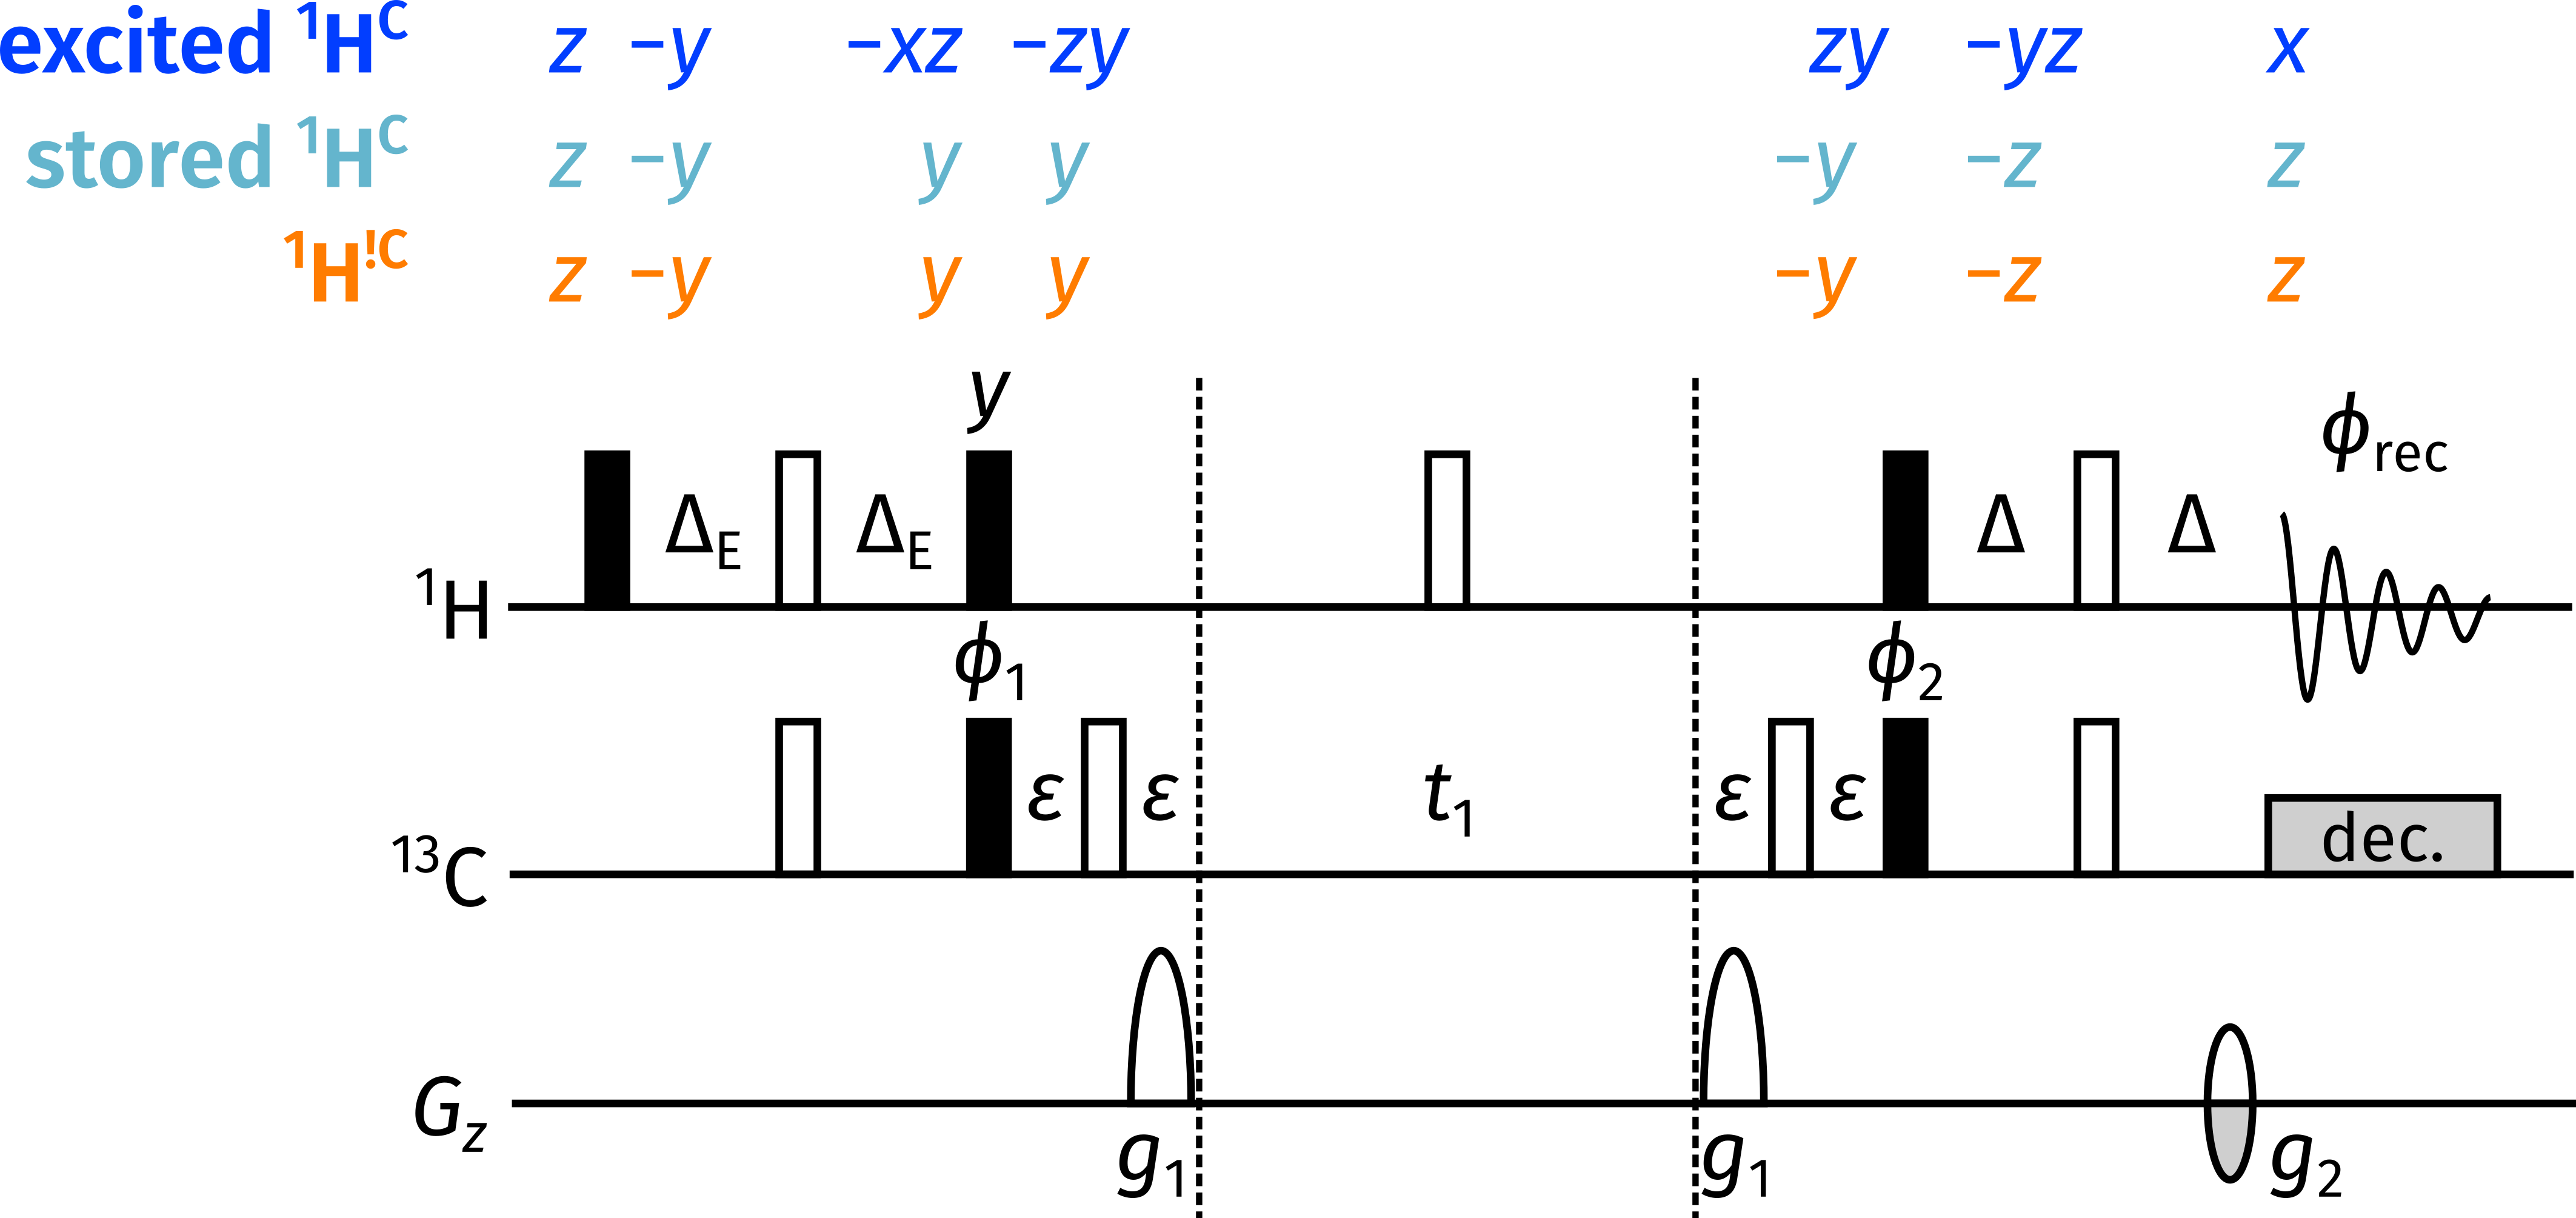
\includegraphics[draft=false]{pp/hsqc/noah_po_inept.png}%
    \caption[NOAH HSQC module with partial excitation product operator analysis]{
        NOAH HSQC module with partial excitation, where the delay $\DeltaE$ is changed from the usual value of $1 / (4J)$.
        As shown by the product operator analysis, proportion $f\/$ of \magn{C} magnetisation is stored along $+z$ at the end of the sequence and can be sampled again in a later module.
        Gradient amplitudes are $(g_1, g_2) = (75\%, \pm 18.9\%)$; all other symbols have the same meaning as in \cref{fig:sehsqc_po}.
        (The different CTP gradient amplitudes are chosen to avoid accidental refocusing between different modules.)
    }
    \label{fig:noah_hsqc_deltae_po}
\end{figure}

In order to accomplish partial \magn{C} excitation in the NOAH HSQC module (\cref{fig:noah_hsqc_deltae_po}), the INEPT delay $\DeltaE$ should be modified from its usual value of $1 / (4J)$ (where $J$ is short for $\oneJ{CH}$).
After the \ang{90}($I$)--$\DeltaE$--\ang{180}($I,S$)--$\DeltaE$ INEPT block, the relevant product operators are
\begin{equation}
    \label{eq:inept_changed}
    \cos(2\pi J\DeltaE) I_y - \sin(2\pi J\DeltaE) 2I_xS_z.
\end{equation}
In a `normal' INEPT block, the choice of $\DeltaE = 1/(4J)$ makes the cosine term vanish, leaving us with only the term $-2I_xS_z$.
Since this term is subsequently transferred to spin $S\/$ and labelled in $t_1$, this choice of $\DeltaE = 1/(4J)$ corresponds to \textit{complete} excitation of \magn{C} magnetisation.

However, if we choose $\DeltaE < 1/(4J)$, then the first $I_y$ term---which corresponds to `stored' or unexcited \magn{C} magnetisation---is eventually returned to $I_z$, as shown by the product operator analysis in \cref{fig:noah_hsqc_deltae_po}.%
\footnote{In the context of the ASAP experiments (both HMQC and HSQC), this is termed \textit{Ernst angle} excitation because the unexcited magnetisation is stored for later repetitions of the \textit{same} experiment, which mirrors the original Ernst angle for the 1D pulse--acquire experiment.
However, for NOAH supersequences, the magnetisation is stored for other modules, so it is more correct to refer to this as a \textit{partial} excitation.}
To be precise, in order to excite a fraction $f\/$ of \magn{C} magnetisation (and store the remaining $(1 - f)$ for the next module), we require that
\begin{equation}
    \label{eq:ssc_inept_delay}
    \DeltaE = \frac{2\Delta \arcsin f}{\pi},
\end{equation}
where $\Delta$ is the usual value of $1/(4J)$.
The spectra obtained from a \noah{S,S,Cc} supersequence, using this partial \magn{C} excitation in the first HSQC module (with $f = 0.8$), are shown in \cref{fig:sscc_example}.

\begin{figure}[!ht]
    \centering
    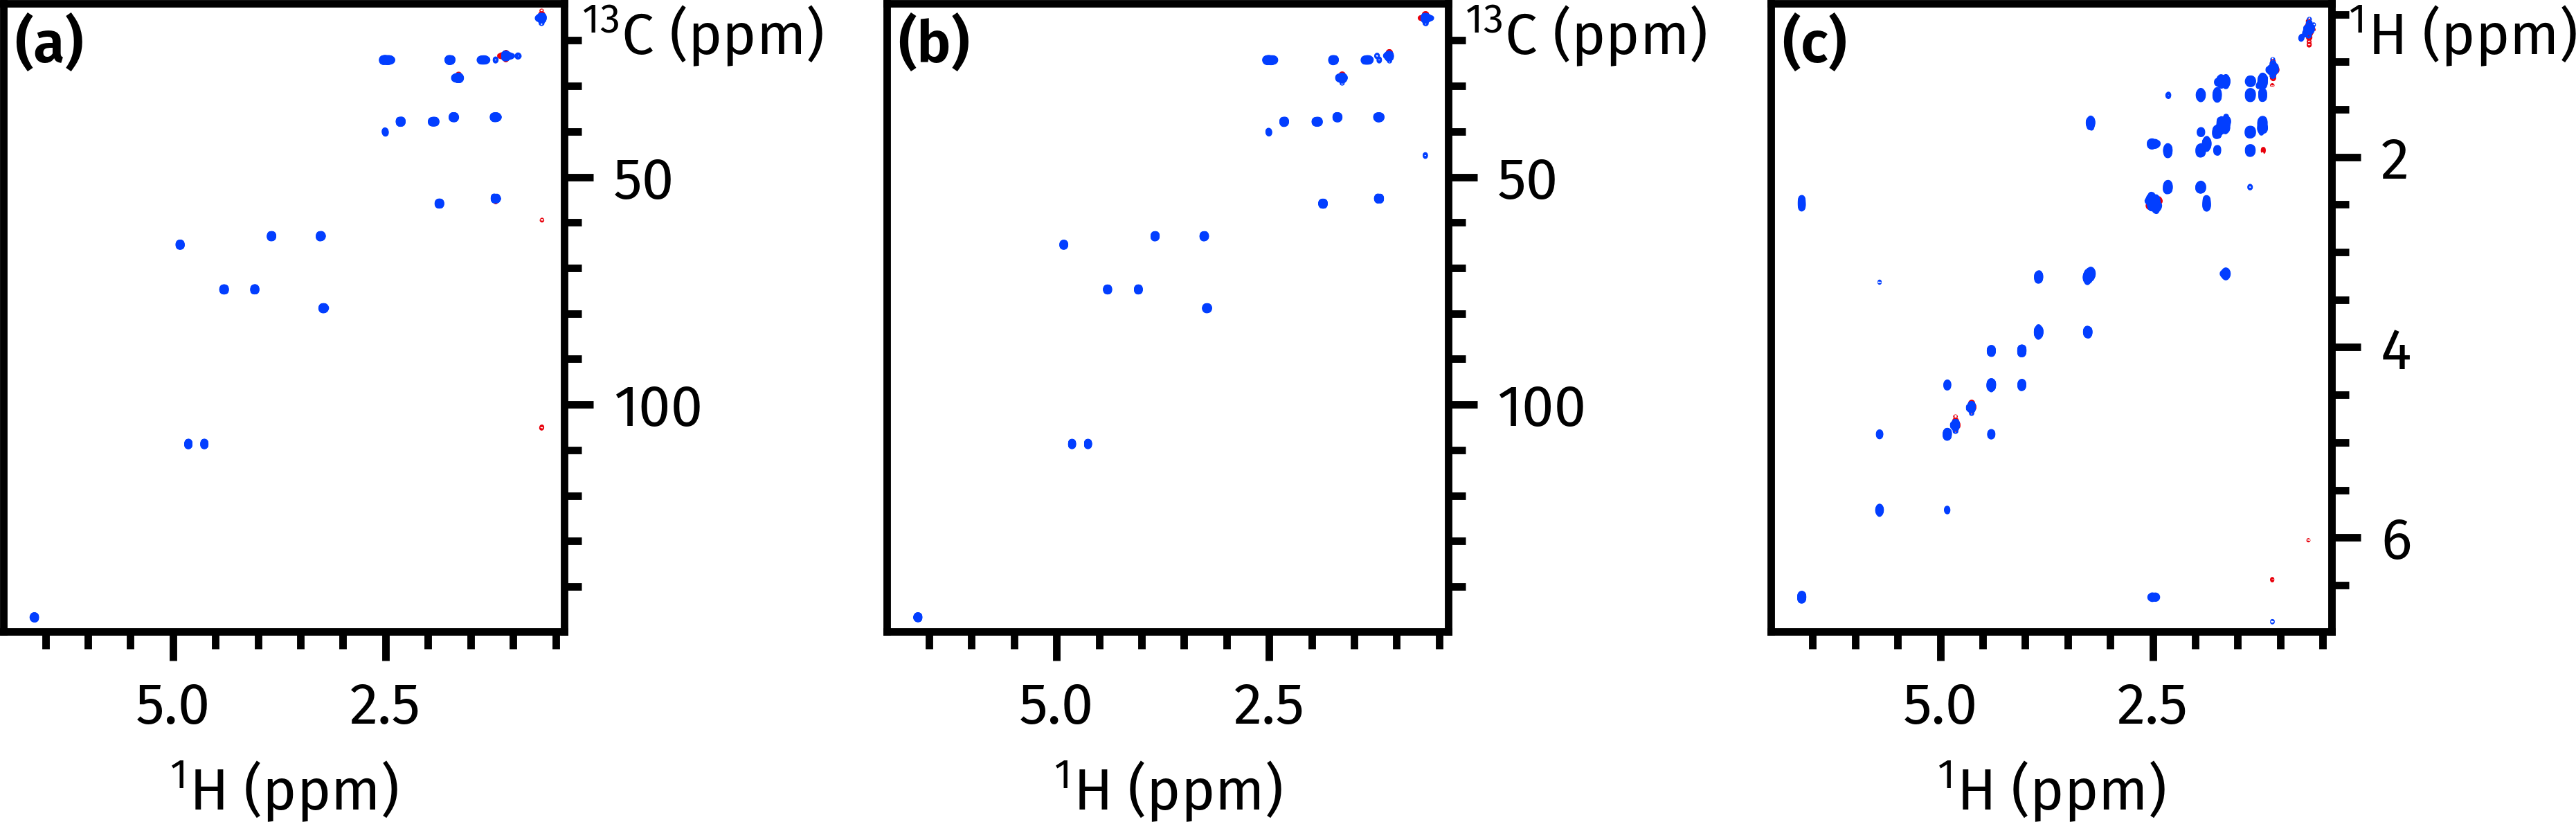
\includegraphics[draft=false]{noah/sscc_example.png}%
    {\phantomsubcaption\label{fig:sscc_example_s1}}%
    {\phantomsubcaption\label{fig:sscc_example_s2}}%
    {\phantomsubcaption\label{fig:sscc_example_cc}}%
    \caption[Spectra from \noah{S,S,Cc} supersequence]{
        Spectra from a \noah{S,S,Cc} supersequence, where the INEPT delay of the first HSQC module was modified to only excite a fraction $f = 0.8$ of \magn{C} magnetisation.
        \textbf{(\subref*{fig:sscc_example_s1})} First HSQC.
        \textbf{(\subref*{fig:sscc_example_s2})} Second HSQC.
        \textbf{(\subref*{fig:sscc_example_cc})} CLIP-COSY.
        \datacode{7A-201010}
    }
    \label{fig:sscc_example}
\end{figure}

In \cref{fig:sscc_improvements_base}, the intensities of these spectra are compared against the HSQC and CLIP-COSY in a \noah{S,Cc} supersequence.
As expected, the first HSQC retains (around) 80\% of its `base' sensitivity, corresponding to the fraction of excited magnetisation.
The second HSQC spectrum \textit{nominally} only has access to the remaining 20\% of magnetisation: however, due to recovery of \magn{C} magnetisation during the FID of the first HSQC, this number is boosted to 65\%.
The CLIP-COSY sensitivity is (very slightly) decreased compared to a \noah{S,Cc} supersequence: this is because of cumulative losses from the two HSQC modules.

\Cref{fig:sscc_improvements_sehsqc,fig:sscc_improvements_dipsi,fig:sscc_improvements_split_sehsqc} detail several possible modifications to this basic scheme.
In the first of these (\cref{fig:sscc_improvements_sehsqc}), we further increase the sensitivity of the second HSQC module by converting it into a seHSQC2 module.%
\footnote{The sensitivity increases are not uniform because they depend on multiplicity.}
The CLIP-COSY sensitivity is slightly decreased due to poorer \magnnot{C} preservation, which is consistent with \cref{subsec:noah__sehsqc_c}.
Note, however, that it is not possible to change the \textit{first} HSQC into a seHSQC experiment: none of the seHSQC versions discussed in \cref{subsec:noah__sehsqc_c} preserve unused \magn{C} magnetisation in the same way as the HSQC module above.

\begin{figure}[!ht]
    \centering
    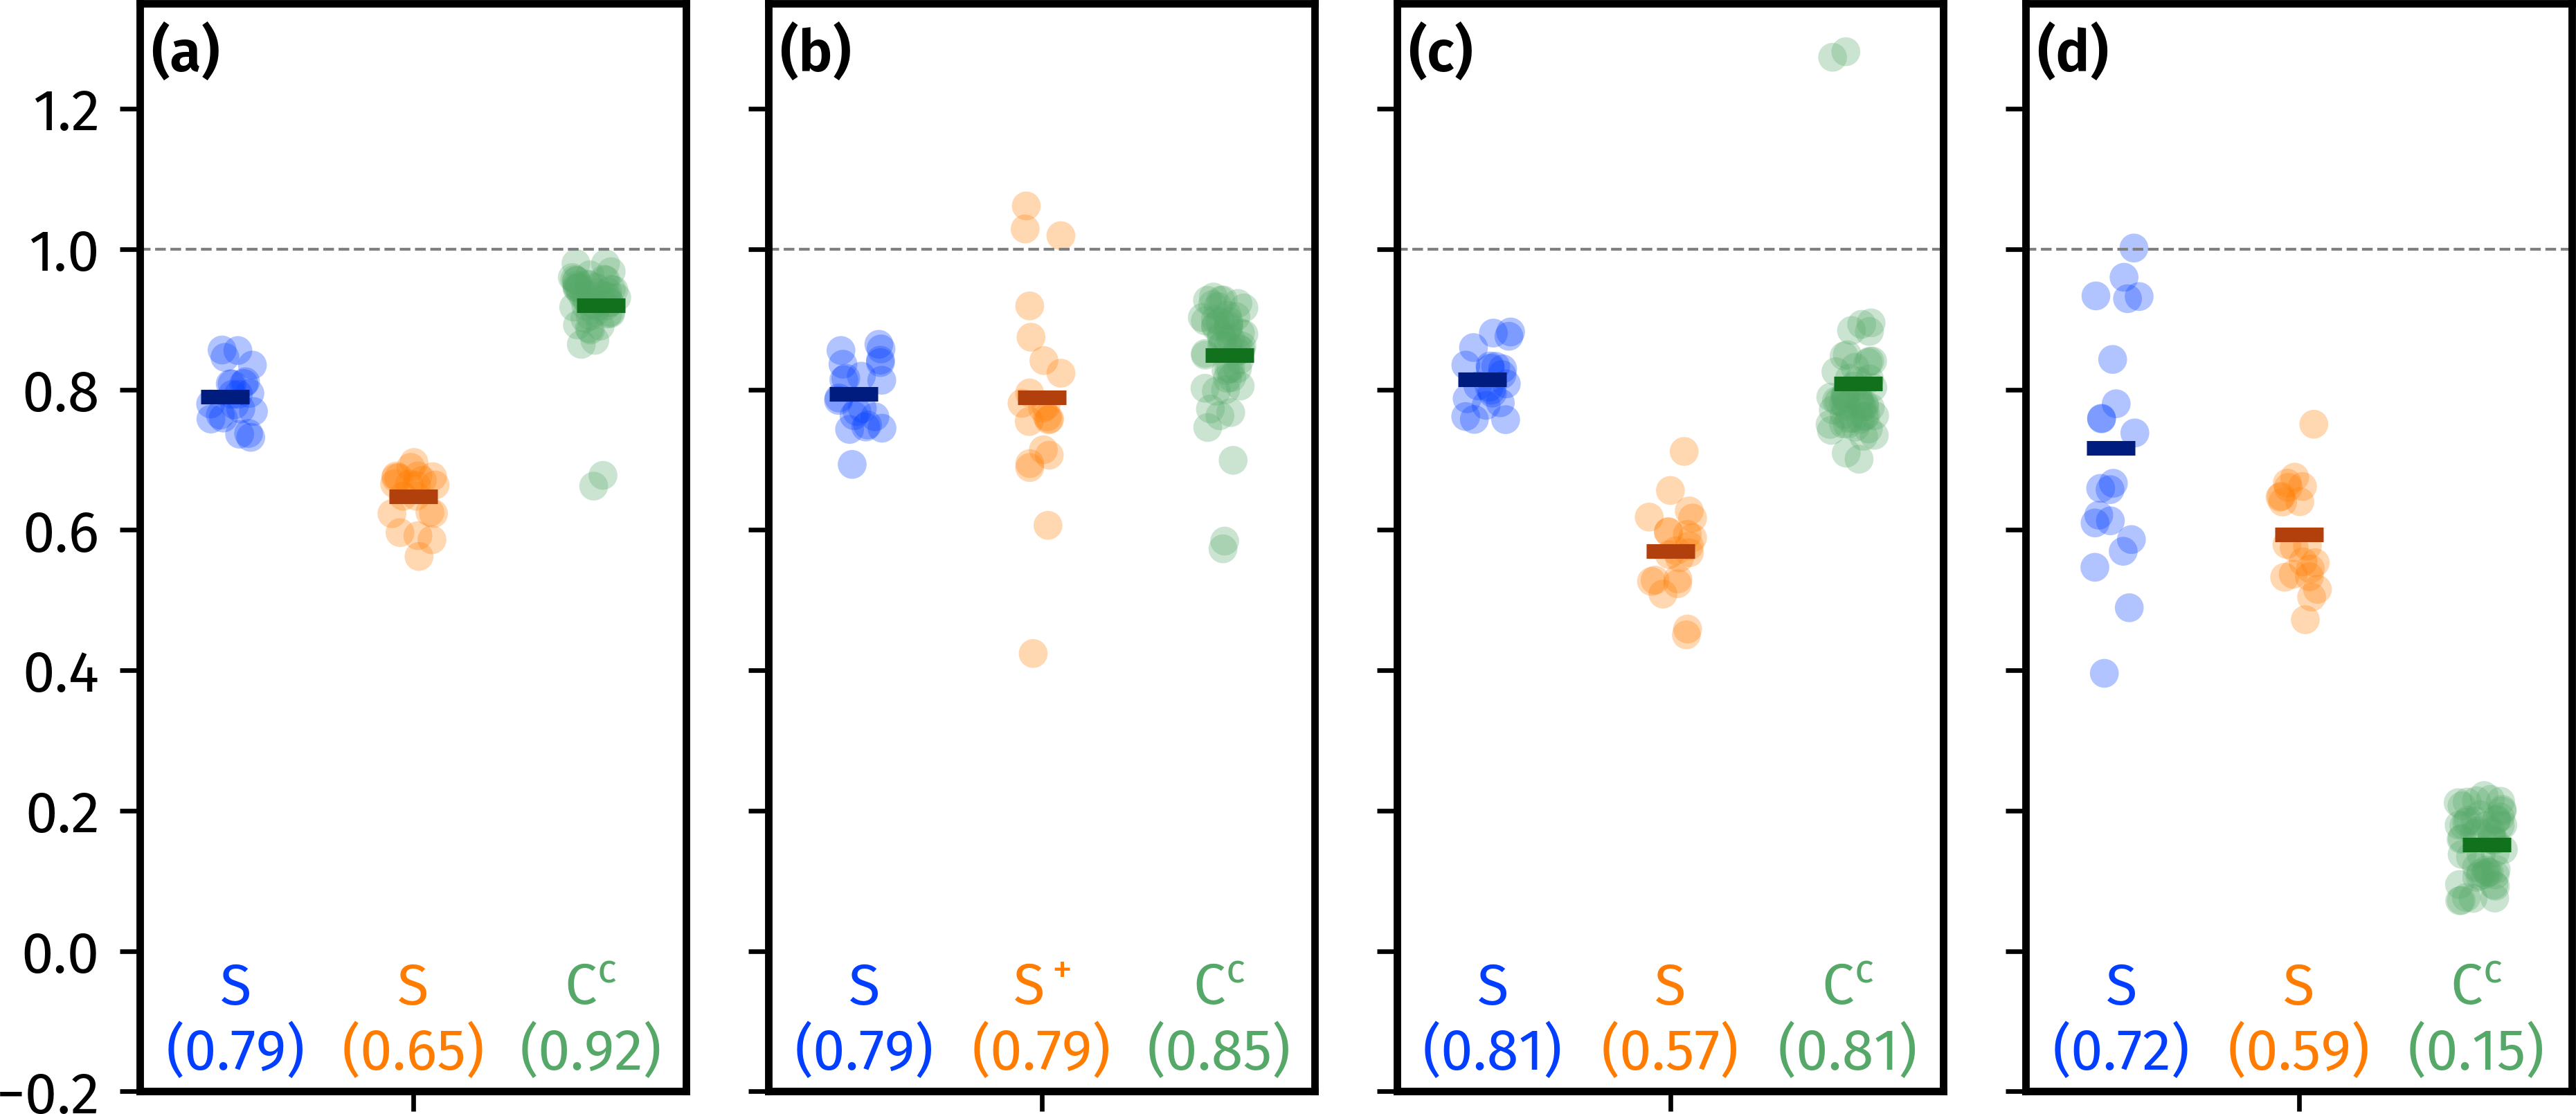
\includegraphics[draft=false]{noah/sscc_improvements.png}%
    {\phantomsubcaption\label{fig:sscc_improvements_base}}%
    {\phantomsubcaption\label{fig:sscc_improvements_sehsqc}}%
    {\phantomsubcaption\label{fig:sscc_improvements_dipsi}}%
    {\phantomsubcaption\label{fig:sscc_improvements_split_sehsqc}}%
    \caption[Sensitivity comparisons for \noah{S,S,Cc} and \noah{S,Sp,Cc} supersequences]{
        Comparisons of HSQC and CLIP-COSY sensitivities of \noah{S,S,Cc} and \noah*{S,Sp,Cc} supersequences.
        The three groups of dots in each subplots refer to the three respective modules in the supersequence.
        Peak intensities are normalised against the HSQC and CLIP-COSY experiments in a \noah{S,Cc} supersequence.
        \textbf{(\subref*{fig:sscc_improvements_base})} \noah{S,S,Cc} with $f = 0.8$ (the same spectra as shown in \cref{fig:sscc_example}).
        \textbf{(\subref*{fig:sscc_improvements_sehsqc})} \noah{S,Sp,Cc} with $f = 0.8$.
        \textbf{(\subref*{fig:sscc_improvements_dipsi})} \noah{S,S,Cc} with $f = 0.8$, plus \qty{35}{\ms} DIPSI-2 mixing after the first HSQC module.
        \textbf{(\subref*{fig:sscc_improvements_split_sehsqc})} A \noah{S,S,Cc} supersequence, but using the split-seHSQC implementation of Nolis et al.\autocite{Nolis2019CPC} (as opposed to the ASAP-HSQC module) for the double HSQC.
        \datacode{7A-201010}
    }
    \label{fig:sscc_improvements}
\end{figure}

Alternatively, it is also possible to include a period of isotropic mixing between the two HSQC modules: here, the DIPSI-2 sequence\autocite{Shaka1988JMR} was chosen.
Since the \magn{C} magnetisation pool has been (partially) depleted, and the \magnnot{C} magnetisation pool is (almost) full, this should in theory lead to transfer of polarisation from the \magnnot{C} pool to \magn{C}.
However, when tested, this was not found to have a beneficial impact: in fact, small \textit{decreases} in sensitivity were observed for both the second HSQC module and the final CLIP-COSY (\cref{fig:sscc_improvements_dipsi}).

\begin{figure}[!ht]
    \centering
    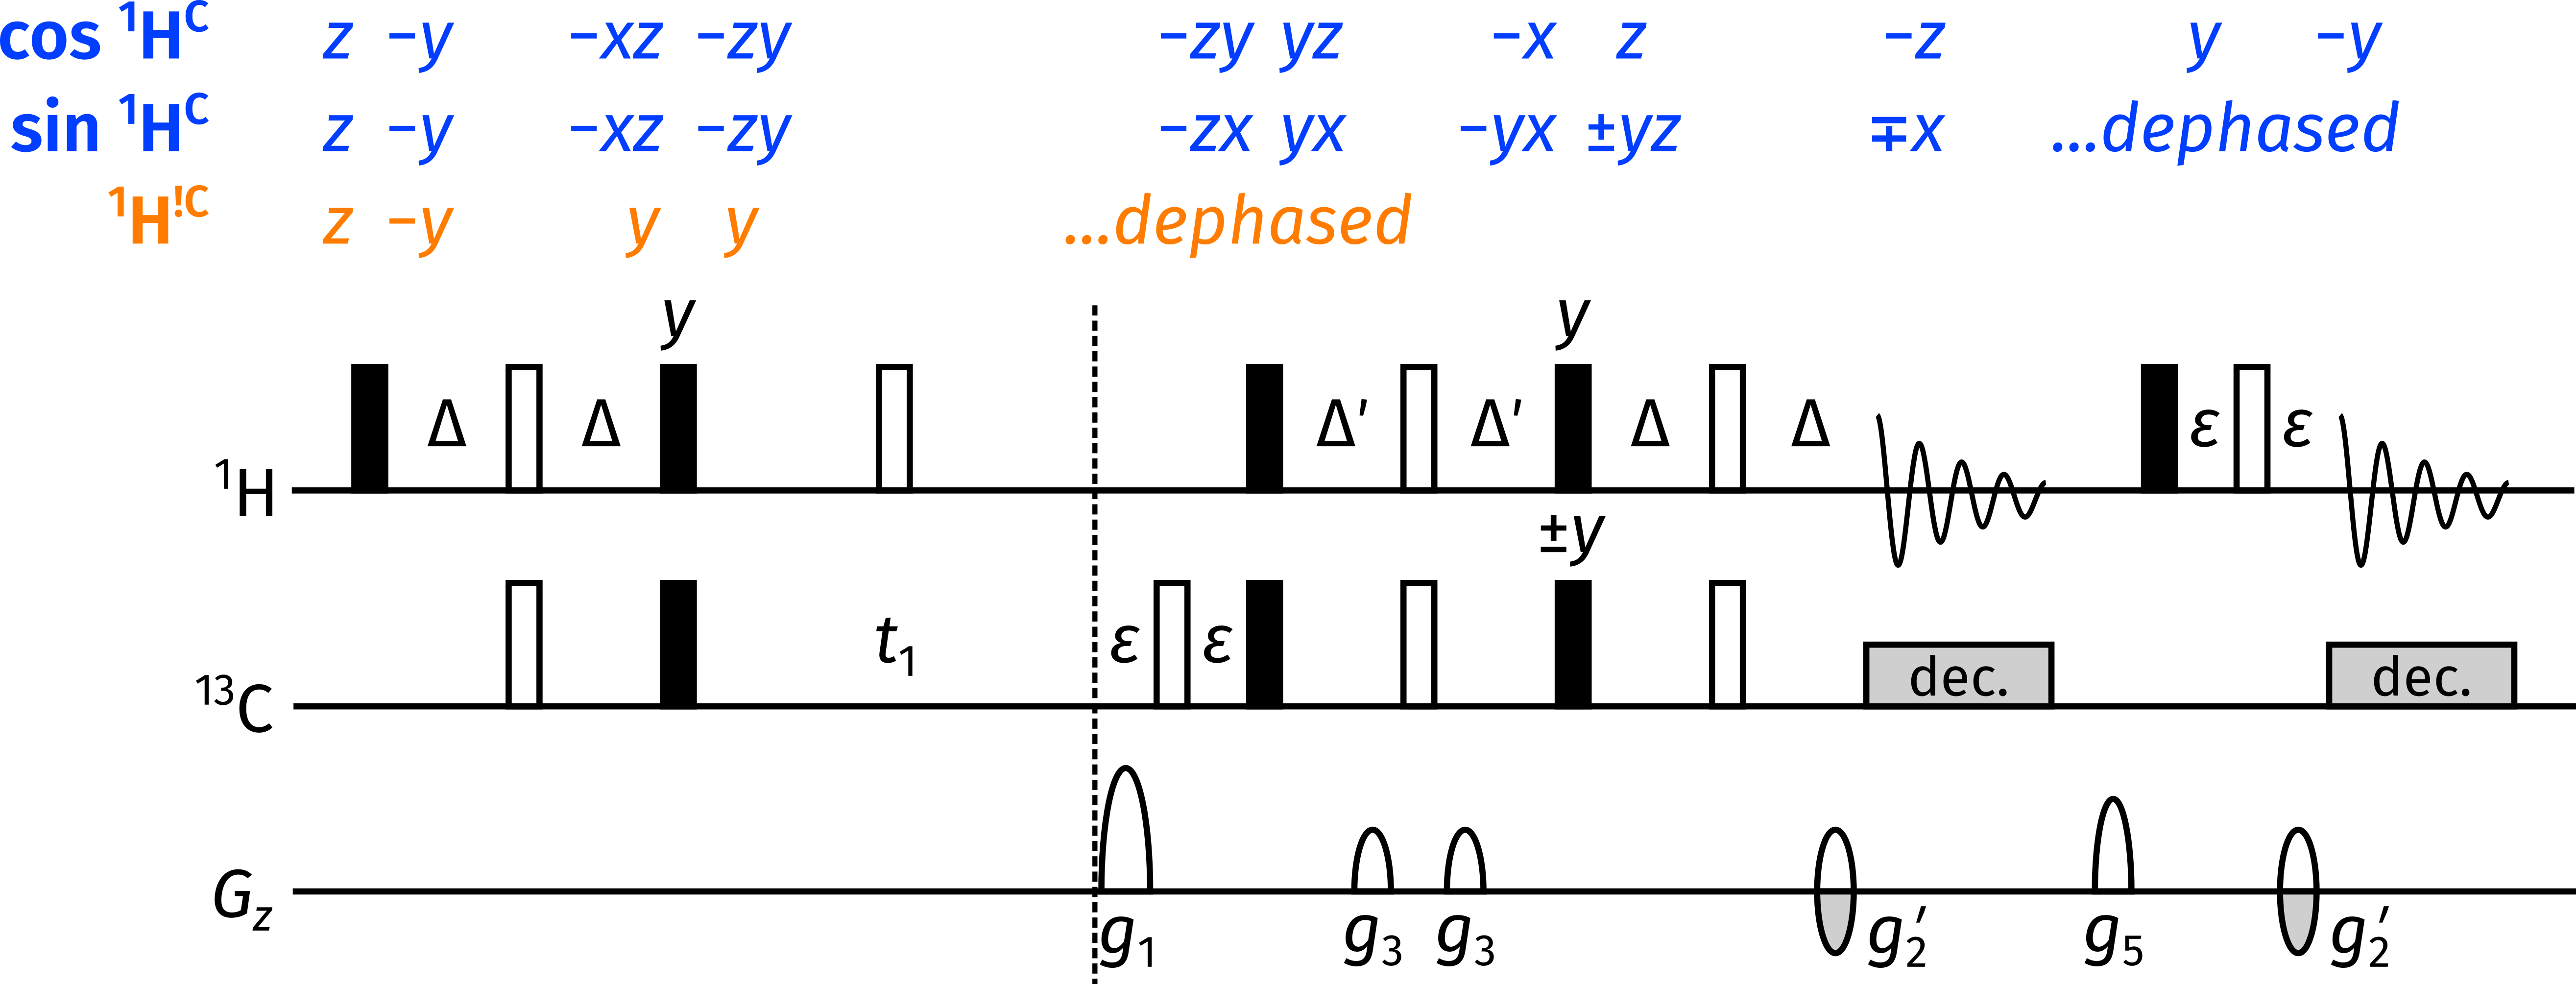
\includegraphics[draft=false]{pp/sehsqc/split_crk.png}%
    \caption[Split-seHSQC experiment]{
        Split-seHSQC experiment used for the collection of two HSQC spectra.\autocite{Nolis2019CPC}
        All symbols have the same meaning as in \cref{fig:sehsqc_po_crk}; $g_5$ is a purge gradient with arbitrary amplitude.
    }
    \label{fig:split_crk}
\end{figure}

Lastly, it should also be noted that the acquisition of two HSQC spectra in one experiment has also been accomplished in a different way by Parella and coworkers\autocite{Nolis2019CPC,Nolis2019JMR}.
This relies on `splitting' up the CRK seHSQC experiment (\cref{fig:sehsqc_po_crk}), such that the cosine- and sine-modulated components are separately detected.%
\footnote{In my paper\autocite{Yong2021JMR}, this was referred to as an `MFA' (multiple-FID acquisition) implementation. I refrain from using this term here because it is ambiguous---after all, NOAH experiments are also multiple-FID experiments.}
This can be easily accomplished by inserting a detection period before the final \proton{} \ang{90} pulse (\cref{fig:split_crk}), where the cosine-modulated component is stored as longitudinal magnetisation and the sine-modulated component is transverse (and in-phase).

However, this implementation does not fare as well in the context of the \noah{S,S,Cc} supersequences investigated here.
The sensitivity of the three modules when using this is shown in \cref{fig:sscc_improvements_split_sehsqc}: the two HSQC spectra have comparable, but slightly poorer, sensitivity than the $f = 0.8$ partial excitation scheme used in \cref{fig:sscc_improvements_base}.
There is also a slightly larger spread in sensitivity, which can be attributed to the fact that the seHSQC does not boost intensities uniformly.
Furthermore, since this experiment (like the parent CRK seHSQC) dephases \magnnot{C} magnetisation, the CLIP-COSY which follows suffers from a large drop in intensity.
Prepending the experiment with the ZIP element to make a `split seHSQC2' does not help, because the bulk magnetisation is in the transverse plane during the first FID.
Finally, the split-seHSQC implementation does not easily allow for features such as multiplicity editing to be independently applied to one of the two signals.%
\footnote{It should at least be \textit{possible} to apply editing to one signal using a modification similar to that done by Nolis et al.\autocite{Nolis2019JMR} However, that is not as simple as the ASAP implementation, where each module is distinct.}

\begin{figure}[!ht]
    \centering
    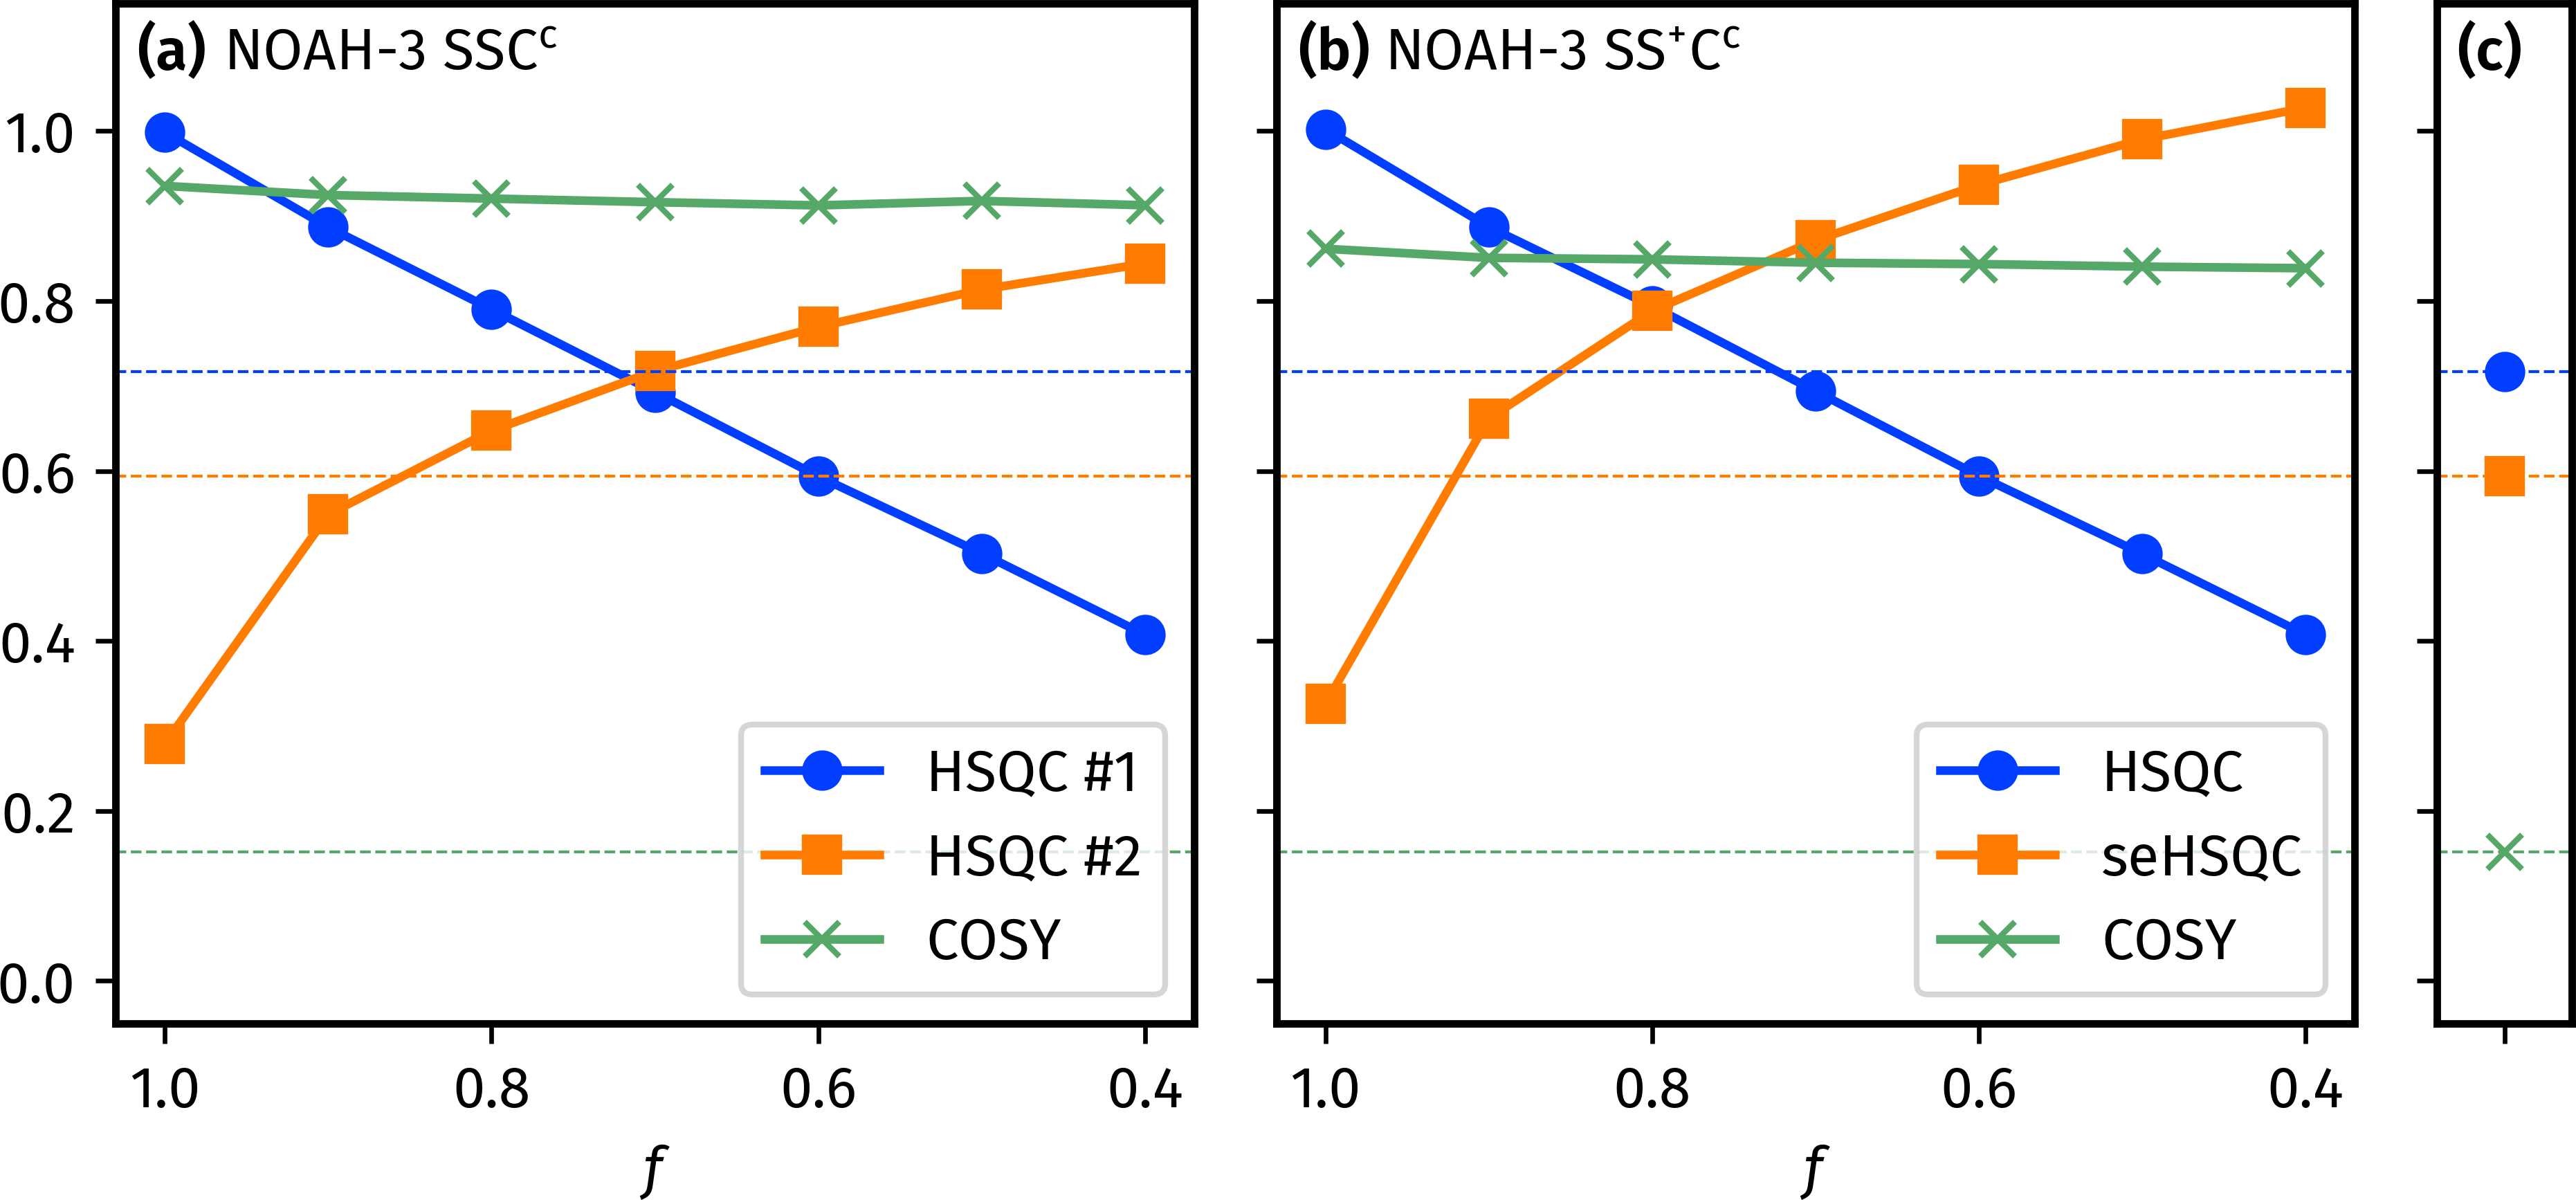
\includegraphics[draft=false]{noah/sscc_comparisons.png}%
    {\phantomsubcaption\label{fig:sscc_comparisons_sscc}}%
    {\phantomsubcaption\label{fig:sscc_comparisons_sspcc}}%
    {\phantomsubcaption\label{fig:sscc_comparisons_split_sehsqc}}%
    \caption[Sensitivity comparisons for \noah{S,S,Cc} and \noah{S,Sp,Cc} supersequences]{
        Sensitivity comparisons for \noah{S,S,Cc} and \noah{S,Sp,Cc} supersequences.
        Intensities are compared against the HSQC and CLIP-COSY modules in a \noah{S,Cc} experiment, and averaged over all peaks.
        \textbf{(\subref*{fig:sscc_comparisons_sscc})} \noah{S,S,Cc} supersequences acquired with different values of $f$.
        \textbf{(\subref*{fig:sscc_comparisons_sspcc})} \noah{S,Sp,Cc} supersequences acquired with different values of $f$.
        \textbf{(\subref*{fig:sscc_comparisons_split_sehsqc})} Using the split-seHSQC implementation.
        \datacode{7A-201010}
    }
    \label{fig:sscc_comparisons}
\end{figure}

\Cref{fig:sscc_comparisons} summarises all of these factors, and further shows how sensitivity varies as a function of the parameter $f$.
From \cref{fig:sscc_comparisons_sscc,fig:sscc_comparisons_sspcc}, it is clear that the sensitivity of the first HSQC is directly proportional to $f$.
The sensitivity of the second HSQC module in \cref{fig:sscc_comparisons_sscc} stems from both the unexcited $(1 - f)$ proportion of \magn{C} magnetisation, plus any that has recovered during the first FID: this latter component decreases as $f\/$ increases.
The CLIP-COSY intensities generally do not vary with $f$.
In \cref{fig:sscc_comparisons_sspcc}, the second HSQC module is replaced with the seHSQC2: this allows $f$ to be increased (from roughly 0.7 to 0.8) in order to obtain spectra with balanced sensitivities.
Finally, for completeness, the split-seHSQC implementation is shown in \cref{fig:sscc_comparisons_split_sehsqc}; the numbers here are the same as in \cref{fig:sscc_improvements_split_sehsqc}.
It is clear that there are several values of $f\/$ which allow the NOAH/ASAP-type implementation to outperform the split-seHSQC experiment in sensitivity.

On its own, the acquisition of two HSQC spectra---as has so far been shown---is not particularly groundbreaking.
However, it is possible to differentiate the two HSQC signals and thereby extract more information.
For example, one spectrum may be run without decoupling in order to measure one-bond coupling constants\autocite{Enthart2008JMR,Nolis2019CPC}; multiplicity editing may be implemented\autocite{SchulzeSunninghausen2017JMR}; or the indirect-dimension spectral width of one of the HSQC spectra can be changed in order to make use of spectral aliasing techniques\autocite{Nolis2019JMR,Jeannerat2011eMR}.
Most interesting of all, though, would be to modify the pulse sequence itself to obtain different \textit{types} of \proton{}--\carbon{} spectra: for example, the addition of an isotropic mixing block to the first HSQC yields an HSQC-TOCSY + HSQC combination\autocite{Nolis2019CPC}, which I now discuss.


\subsubsection{HSQC-TOCSY}

The addition of DIPSI mixing inside the partial-excitation HSQC module leads to an HSQC-TOCSY module (\cref{fig:hsqctocsy_base}), which is (conceptually) identical to the ASAP-HSQC-TOCSY experiment also previously reported by Luy and coworkers\autocite{Becker2019JMR}.
Note that the \proton{} \ang{90} pulse immediately after $t_1$ has a different phase from in the HSQC module: this ensures that \magnnot{C} (and unused \magn{C}) magnetisation is returned to $+z$ after accounting for the extra \ang{180} pulse at the end.

\begin{figure}[!ht]
    \centering
    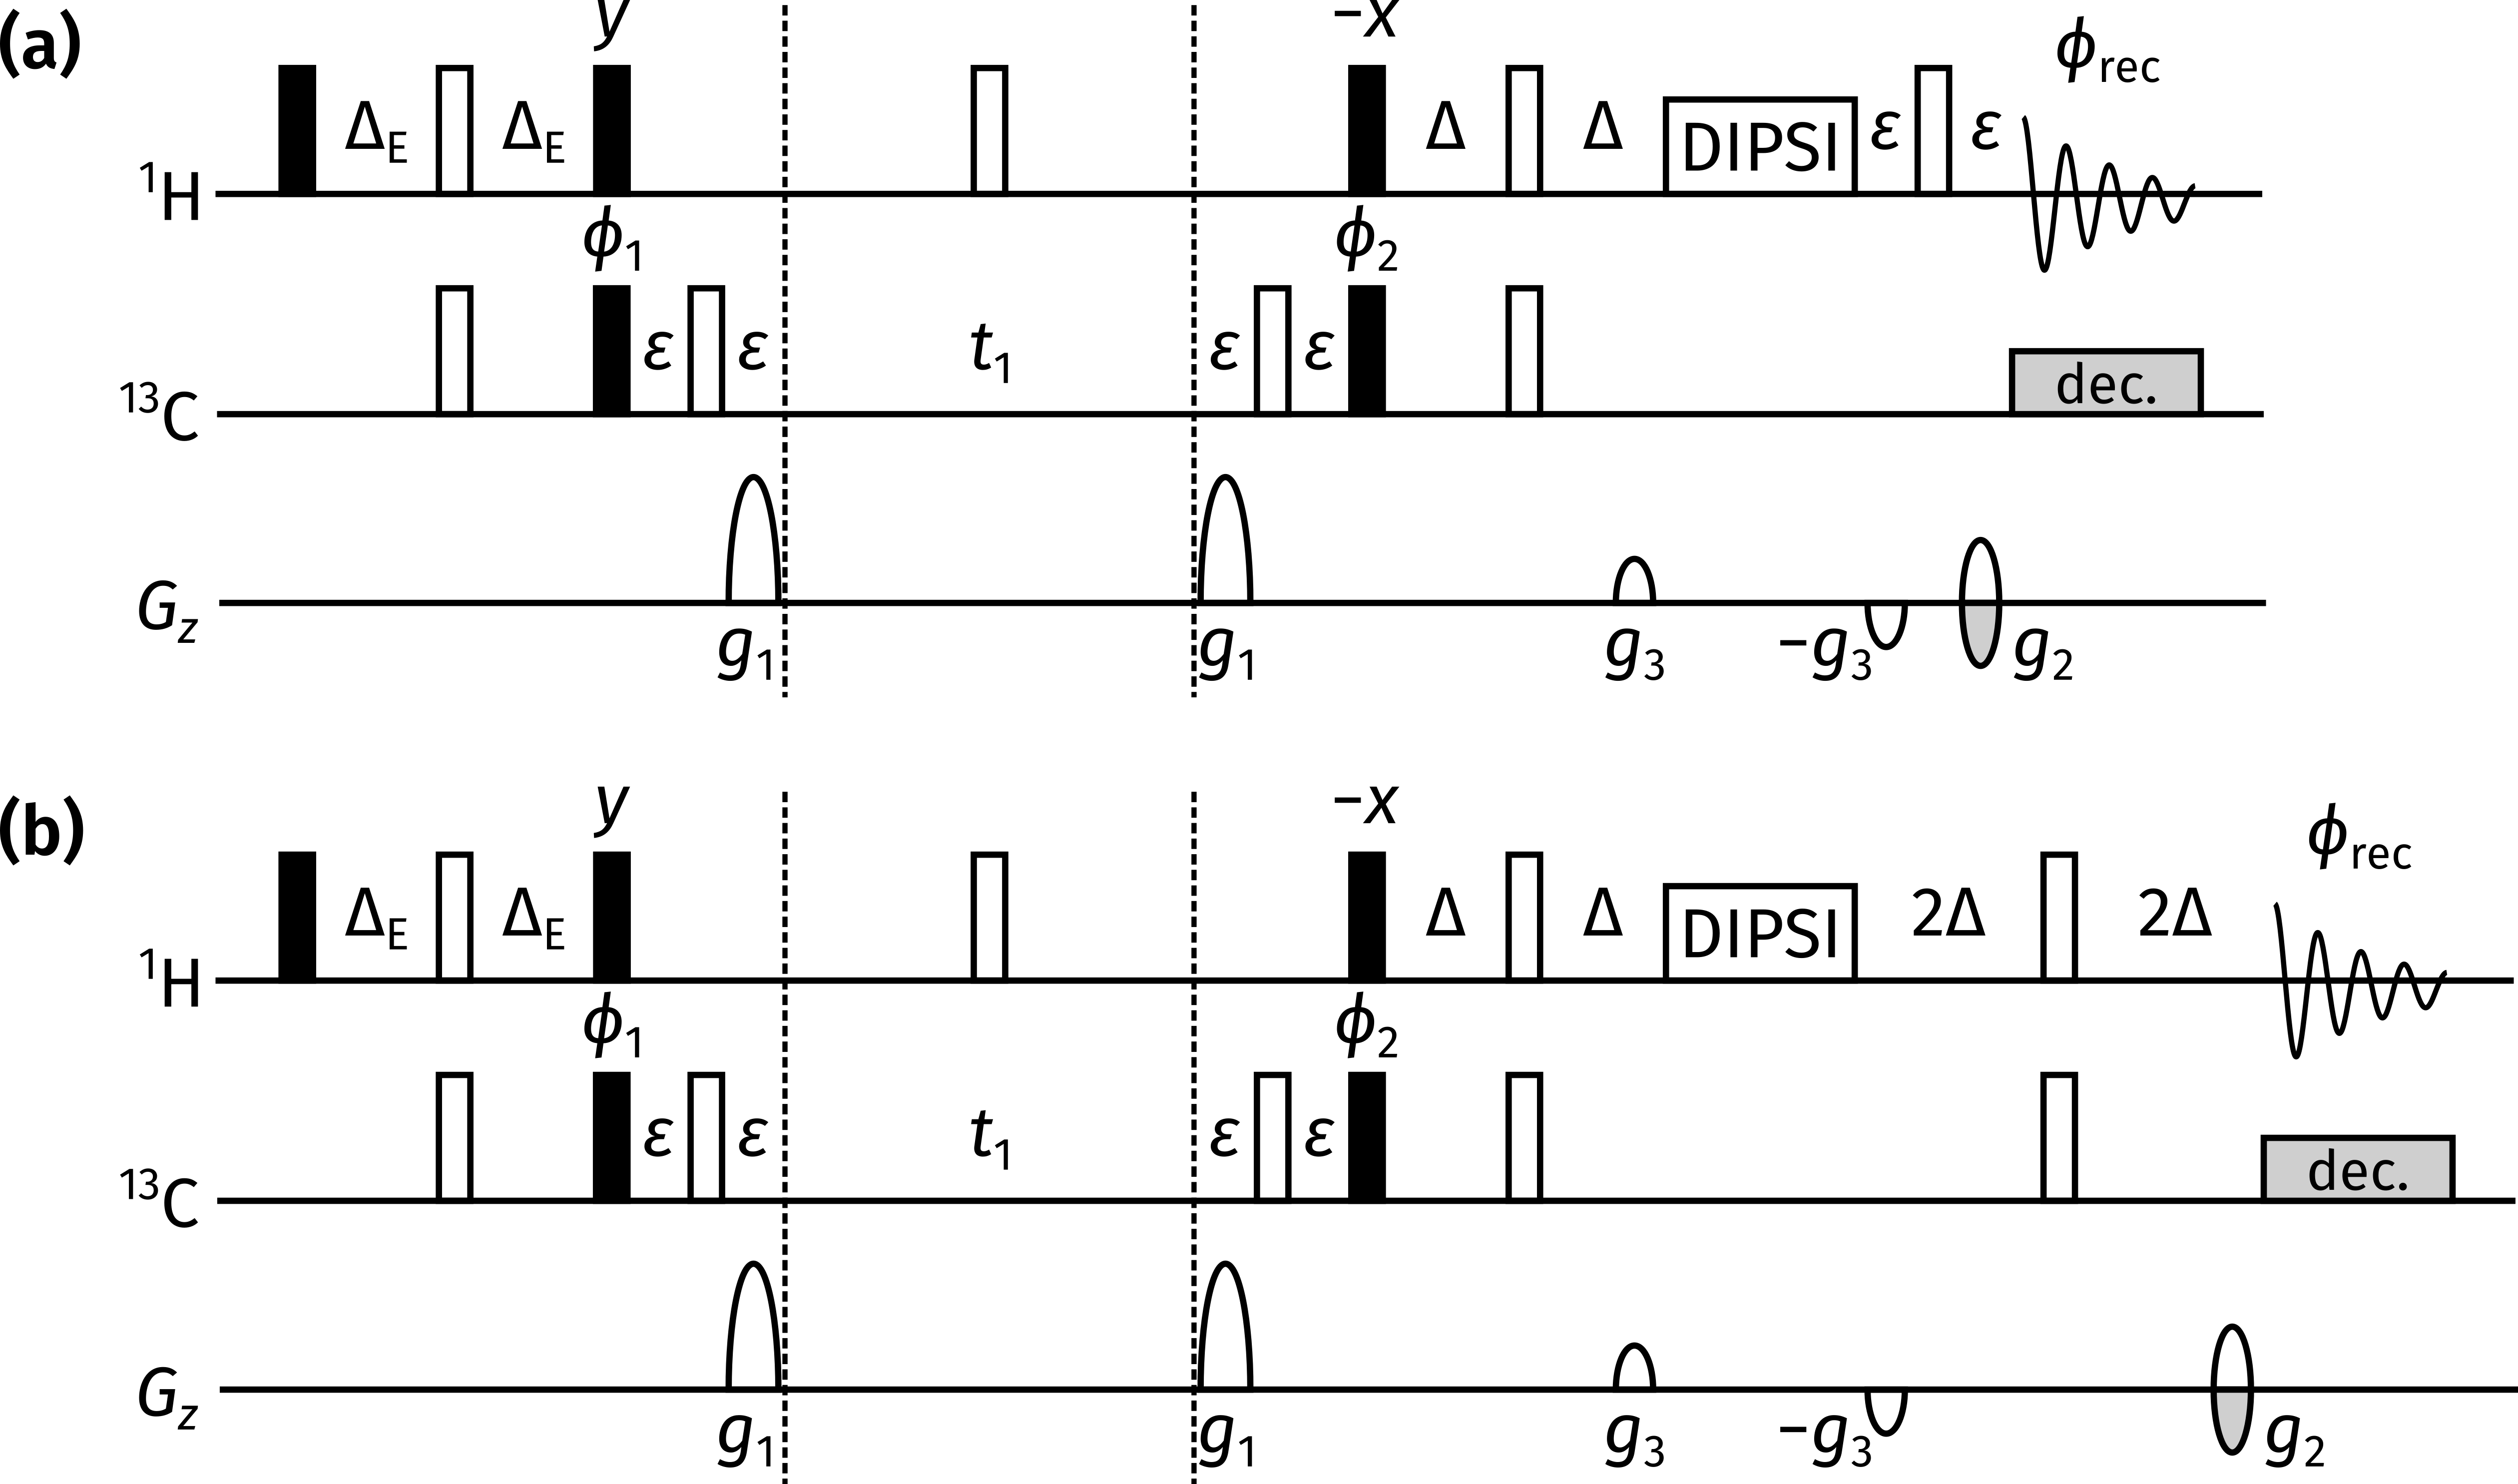
\includegraphics[draft=false]{pp/hsqctocsy.png}%
    {\phantomsubcaption\label{fig:hsqctocsy_base}}%
    {\phantomsubcaption\label{fig:hsqctocsy_invert}}%
    \caption[NOAH HSQC-TOCSY module]{
        NOAH HSQC-TOCSY module:
        \textbf{(\subref*{fig:hsqctocsy_base})} without inversion of HSQC signals (`direct' responses); and
        \textbf{(\subref*{fig:hsqctocsy_invert})} with inversion of HSQC signals.
    }
    \label{fig:hsqctocsy}
\end{figure}

The HSQC-TOCSY module may optionally be implemented with inversion of `direct', HSQC-type responses, which correlate \carbon{} nuclei with directly bonded protons.
This is to be contrasted with the `indirect' responses, which correlate \carbon{} nuclei with other remote protons (in the same spin system), and represent magnetisation which has been transferred during the isotropic mixing period.
This inversion may be accomplished by expanding the final gradient echo to a duration of $4\Delta = 1/J$ (\cref{fig:hsqctocsy_invert}); \carbon{}-bound protons will evolve under $\oneJ{CH}$ and acquire an additional minus sign compared to remote protons.%
\footnote{Of course, the remote protons may also happen to be bonded to \carbon{}, but the chance of this is only $\sim 1\%$.}

The use of such editing in the HSQC-TOCSY is perhaps slightly risky, because it may lead to unwanted peak cancellation through accidental overlap.
Furthermore, if used together with a second HSQC module (as discussed here), this information does not need to be encoded in the HSQC-TOCSY.
Thus, it is not enabled by default; the user must explicitly turn it on through an acquisition flag.
The concept of inverting remote peaks is more important in the HSQC-COSY, which will be discussed in \cref{subsec:noah__hsqccosy}.

\begin{figure}[!ht]
    \centering
    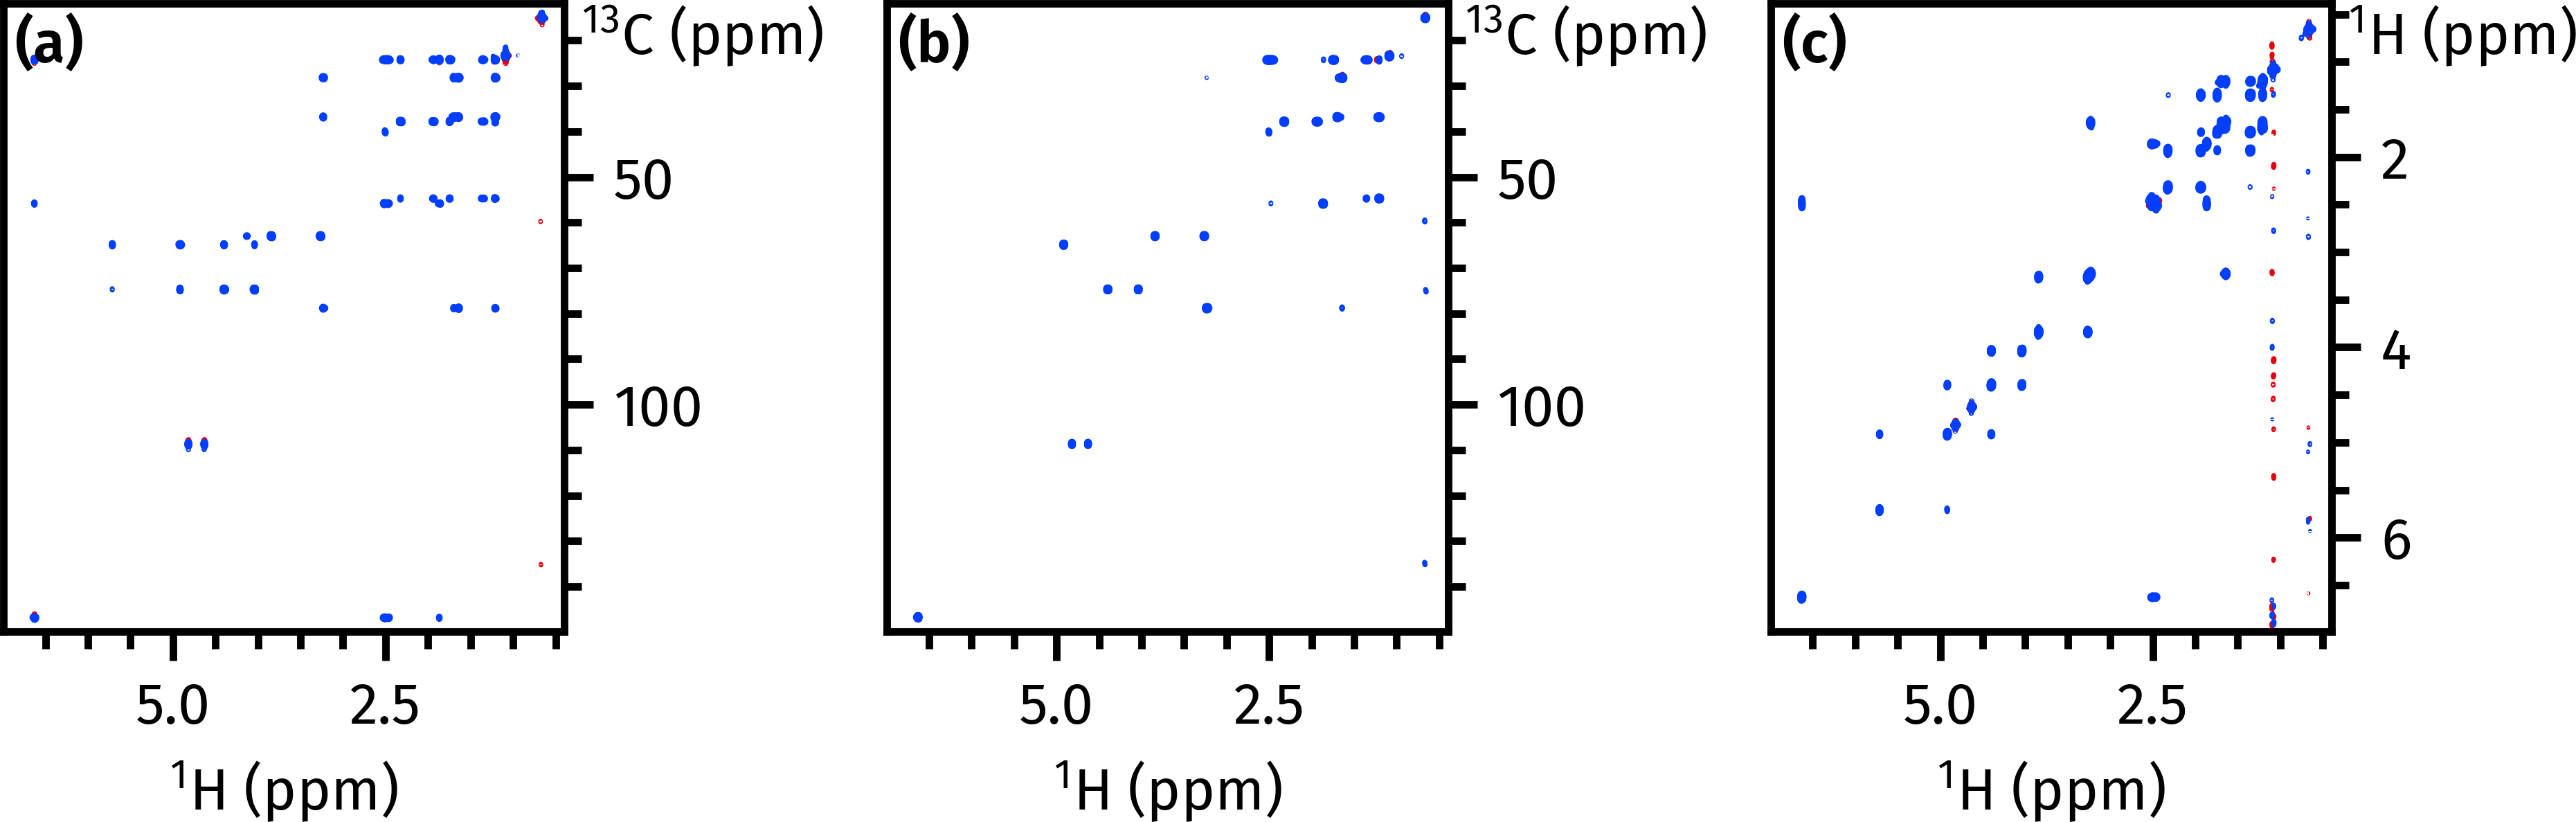
\includegraphics[draft=false]{noah/stspcc_example.png}%
    {\phantomsubcaption\label{fig:stspcc_example_st}}%
    {\phantomsubcaption\label{fig:stspcc_example_sp}}%
    {\phantomsubcaption\label{fig:stspcc_example_cc}}%
    \caption[Spectra from a \noah{St,Sp,Cc} supersequence]{
        Spectra from a \noah{St,Sp,Cc} supersequence.
        \textbf{(\subref*{fig:stspcc_example_st})} HSQC-TOCSY ($f = 0.9$).
        \textbf{(\subref*{fig:stspcc_example_sp})} seHSQC2.
        \textbf{(\subref*{fig:stspcc_example_cc})} CLIP-COSY.
        \datacode{7A-210126}
    }
    \label{fig:stspcc_example}
\end{figure}

With this module in hand, it is possible to implement either \noah{St,S,Cc} or \noah{S,St,Cc} supersequences which yield both HSQC and HSQC-TOCSY data.
In both cases, the first of the two \carbon{} modules can be adjusted to only partially excite \magn{C} magnetisation.
However, the former is preferred as the HSQC-TOCSY has a lower intrinsic sensitivity compared to the HSQC: thus, it is better to place this first in the supersequence, and to also use a larger value of $f\/$ in order to balance the relative sensitivities.
\Cref{fig:stspcc_example} shows an example of the spectra obtained with a setting of $f = 0.9$.

\begin{figure}[!ht]
    \centering
    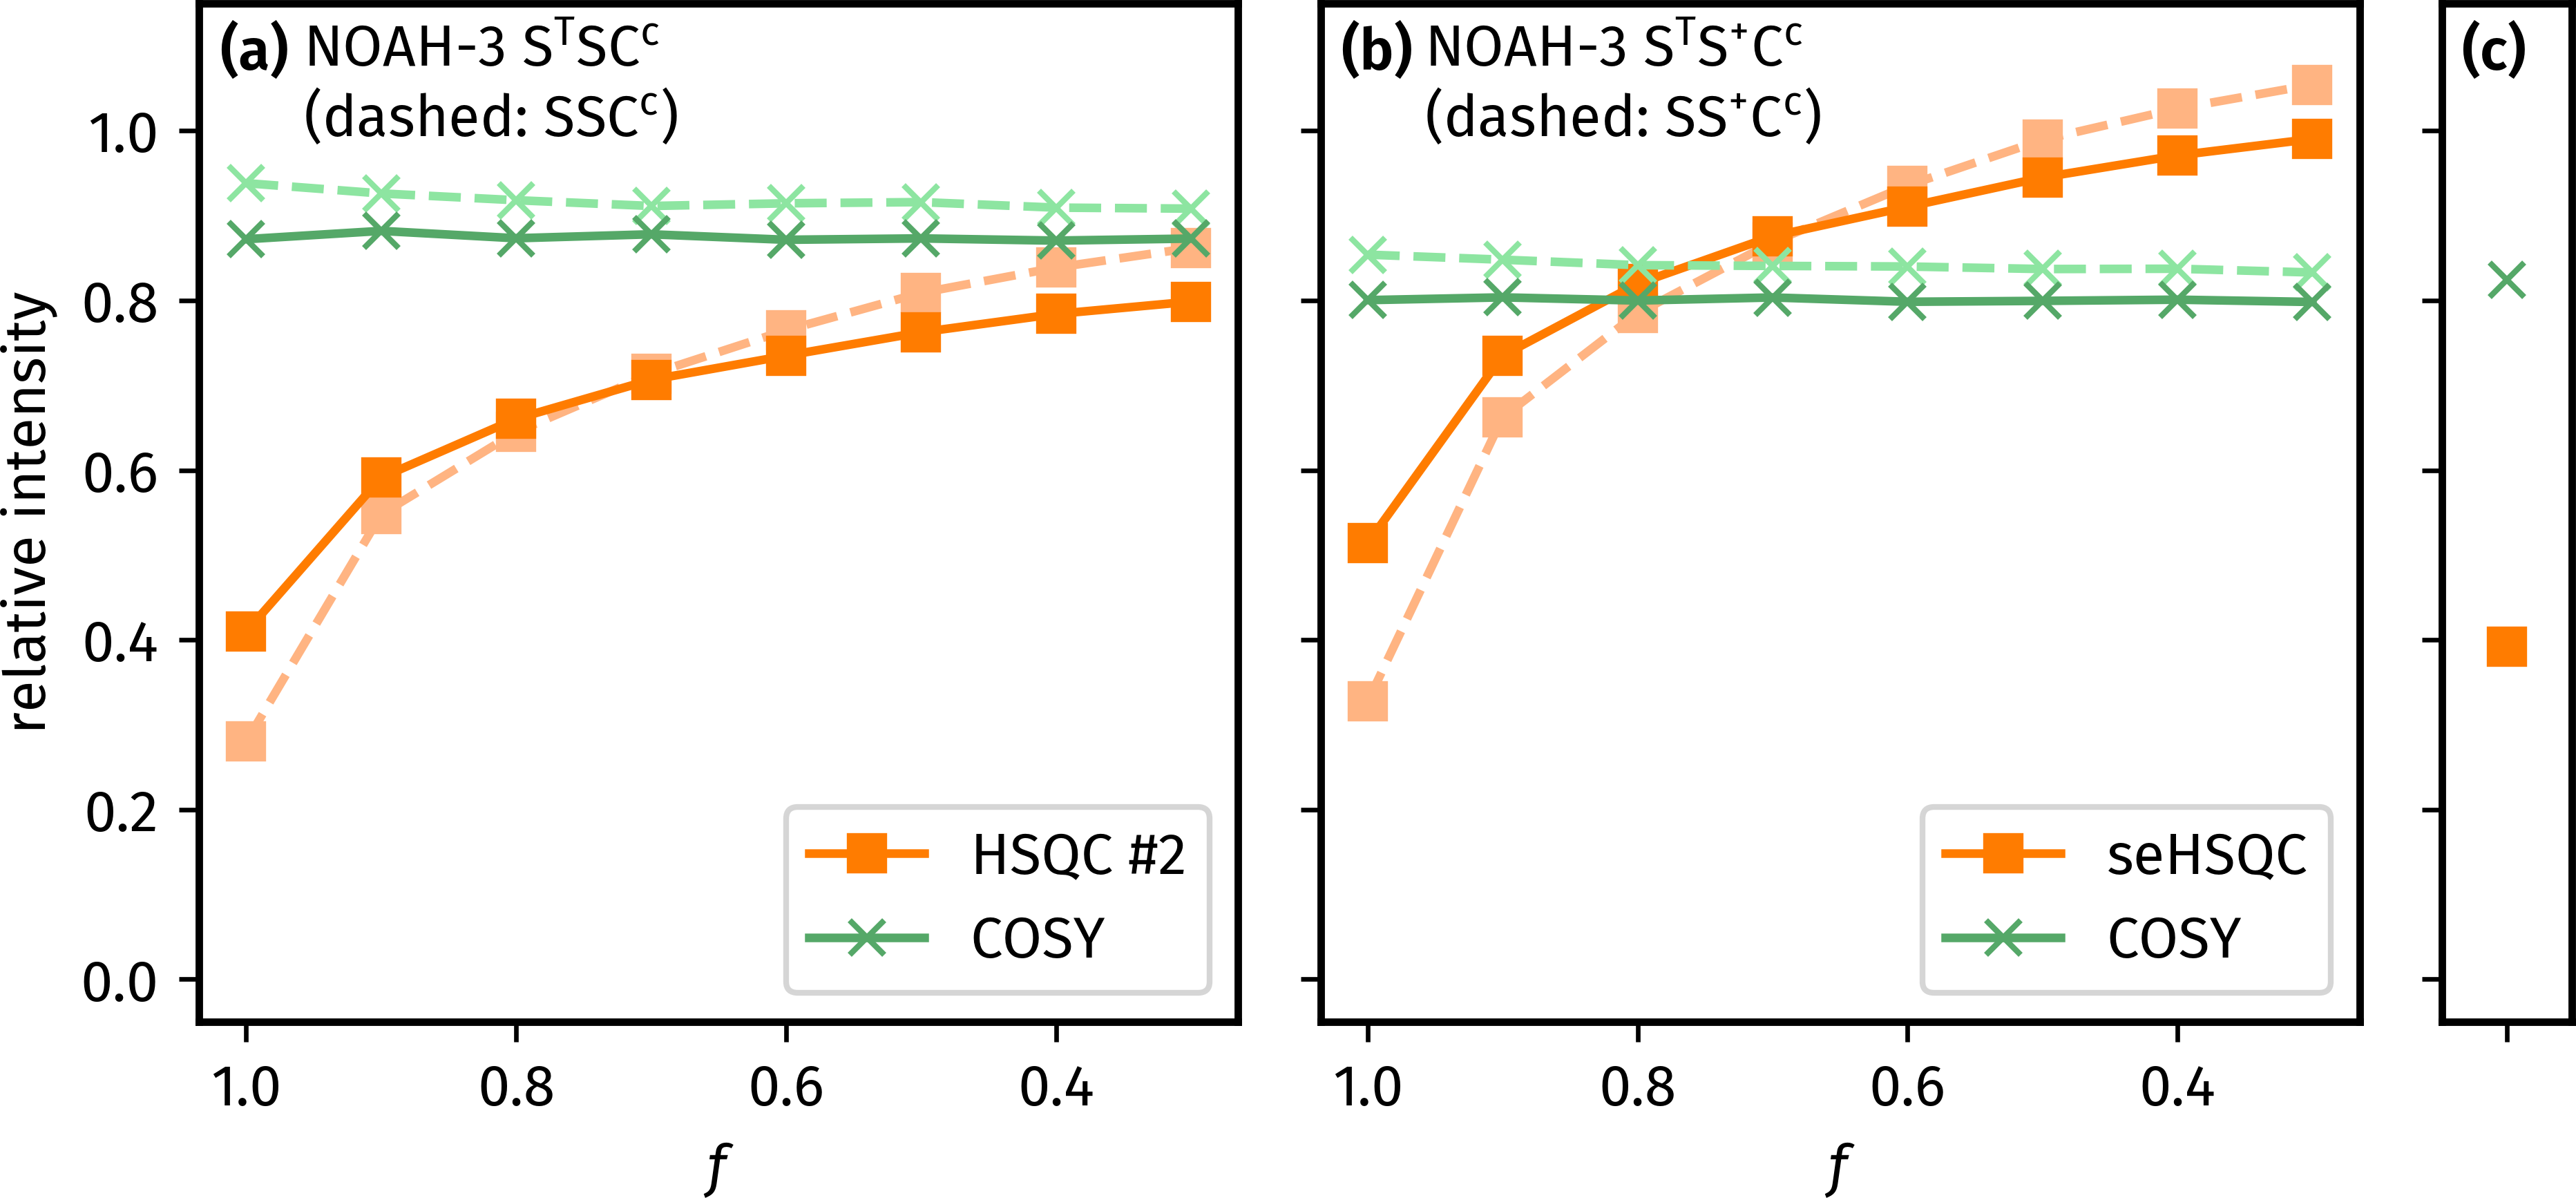
\includegraphics[draft=false]{noah/stscc_comparisons.png}%
    {\phantomsubcaption\label{fig:stscc_comparisons_stscc}}%
    {\phantomsubcaption\label{fig:stscc_comparisons_stspcc}}%
    {\phantomsubcaption\label{fig:stscc_comparisons_sehsqc_tocsy}}%
    \caption[Sensitivity comparisons for supersequences containing HSQC-TOCSY module]{
        Sensitivity comparisons for \noah{S,S,Cc} and \noah{St,S,Cc} supersequences.
        The intensities of the latter two modules are compared against the HSQC and CLIP-COSY modules in a \noah{S,Cc} experiment, and averaged over all peaks.
        \textbf{(\subref*{fig:stscc_comparisons_stscc})} \noah{St,S,Cc} supersequences acquired with different values of $f$; the dashed lines are the corresponding intensities in the \noah{S,S,Cc} supersequence.
        \textbf{(\subref*{fig:stscc_comparisons_stspcc})} The same, but with the seHSQC2 as the second module instead.
        \textbf{(\subref*{fig:stscc_comparisons_sehsqc_tocsy})} The corresponding intensities of the second and third modules in a seHSQC-TOCSY + HSQC + CLIP-COSY supersequence: this is to be compared with the first data point ($f = 1$) in (\subref*{fig:stscc_comparisons_stscc}).
        \datacode{7A-210126}
    }
    \label{fig:stscc_comparisons}
\end{figure}

Finally, I performed a series of experiments to establish whether changing the first module from an HSQC (i.e.\ \noah*{S,S,Cc}) to an HSQC-TOCSY (i.e.\ \noah{St,S,Cc}) would affect the sensitivities of the two latter modules.
The results are shown in \cref{fig:stscc_comparisons_stscc,fig:stscc_comparisons_stspcc}, where the solid lines represent the supersequences starting with the HSQC-TOCSY, and the dashed lines those starting with the HSQC.
At large values of $f\/$ (corresponding to depletion of the \magn{C} pool), the subsequent \carbon{} module experiences sensitivity \textit{gains} when the HSQC-TOCSY is used.
However, this changes at smaller values of $f\/$, where a drop in intensity is instead observed.
For the CLIP-COSY module, the HSQC-TOCSY leads to slightly lower sensitivities across the board.
All of these changes are, however, extremely minor: the supersequences shown here still work entirely as expected.

\Cref{fig:stscc_comparisons_sehsqc_tocsy} shows one final alternative which has not yet been considered: the use of the seHSQC-TOCSY\autocite{Hansen2021AC} as the first module.
This experiment is similar to the seHSQC2 module, but with the addition of isotropic mixing.
Although this fully maximises the intensity of the HSQC-TOCSY component (not shown in \cref{fig:stscc_comparisons}), and also preserves \magnnot{C} magnetisation for the CLIP-COSY (as evidenced by the relatively high CLIP-COSY intensity in \cref{fig:stscc_comparisons_sehsqc_tocsy}), it cannot retain any portion of \magn{C} magnetisation.
Thus, any later module which draws on the same magnetisation pool will only be able to use any signal which has recovered during the FID, just like in an experiment run with $f = 1$.
In this case, the second module is a plain HSQC (not seHSQC): thus, its sensitivity is similar to the leftmost point in \cref{fig:stscc_comparisons_stscc}.
